\chapter{Discussion and results}
\section{Results}
\subsection{Auto CCTV tracking}
All versions were allowed to run for 100 cycles, and the time for each full cycle was logged. One full cycle involves grabbing the image, processing it, finding any glyphs and sending PTZ-commands to the camera. It was also logged how much time was spent on grabbing the image. The mean full cycle time was plotted in the same plot.

\paragraph{C++ only}
The data can be found in appendix \ref{dat:cppfullcycle} on \pageref{dat:cppfullcycle}.

\begin{itemize}
\item Mean: 43.6120 milliseconds
\item Std Dev: 3.7799 milliseconds
\item Minium: 38.0935 milliseconds
\item Maximum: 176.378 milliseconds
\end{itemize}

\begin{figure}[ht]
    \centering
    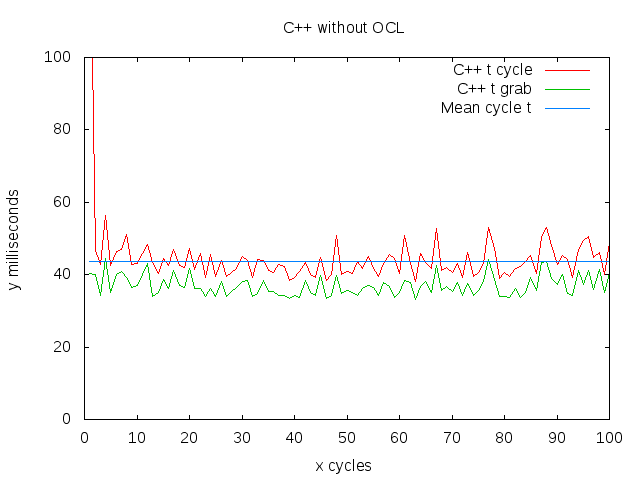
\includegraphics[width=1.0\textwidth]{output_cpp.png}
    \caption{Cycle timing for pure C++ version. Source: Own work, data in \ref{dat:cppfullcycle}}
    \label{fig:output_cpp}
\end{figure}
\FloatBarrier

\paragraph{C++ and OpenCL}
The data can be found in appendix \ref{dat:cppoclfullcycle} on \pageref{dat:cppoclfullcycle}.
\begin{itemize}
\item Mean: 44.3577 milliseconds
\item Std Dev: 4.7298 milliseconds
\item Minium: 37.0841 milliseconds
\item Maximum: 147.944 milliseconds
\end{itemize}

\begin{figure}[ht]
    \centering
    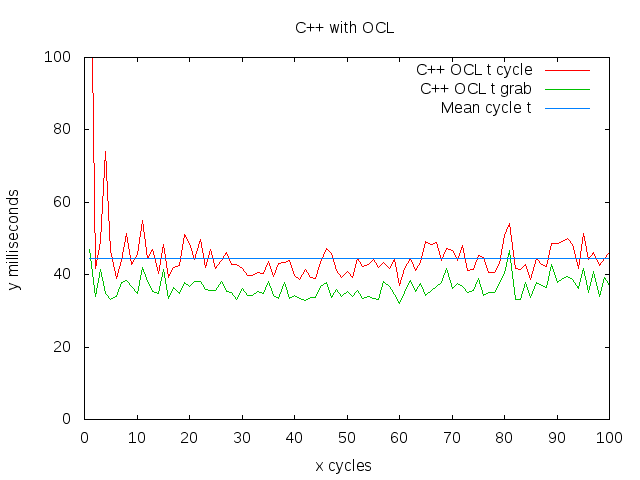
\includegraphics[width=1.0\textwidth]{output_cpp_ocl.png}
    \caption{Cycle timing for C++ and OpenCL version. Source: Own work, data in \ref{dat:cppoclfullcycle}}
    \label{fig:output_cpp_ocl}
\end{figure}
\FloatBarrier

\paragraph{Python}
The data can be found in appendix \ref{dat:cppoclfullcycle} on \pageref{dat:cppoclfullcycle}.

\begin{itemize}
\item Mean: 8302.39 milliseconds
\item Std Dev: 31.9534 milliseconds
\item Minium: 8270.0 milliseconds
\item Maximum: 8535.0 milliseconds
\end{itemize}

\begin{figure}[ht]
    \centering
    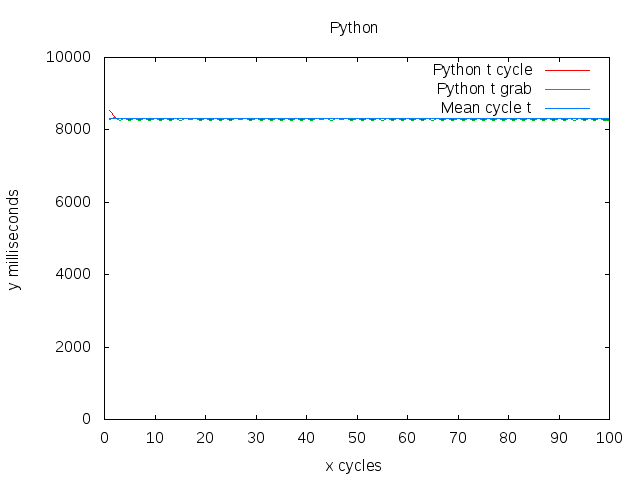
\includegraphics[width=1.0\textwidth]{output_py.png}
    \caption{Cycle timing for Python version. Source: Own work, data in \ref{dat:cppoclfullcycle}}
    \label{fig:output_cpp_ocl}
\end{figure}
\FloatBarrier



\subsection{Tubular detection}
The tubular detection proof of concept provided output with colored overlays. The pink circles represents a tubular that has been detected.

\begin{figure}[ht]
    \centering
    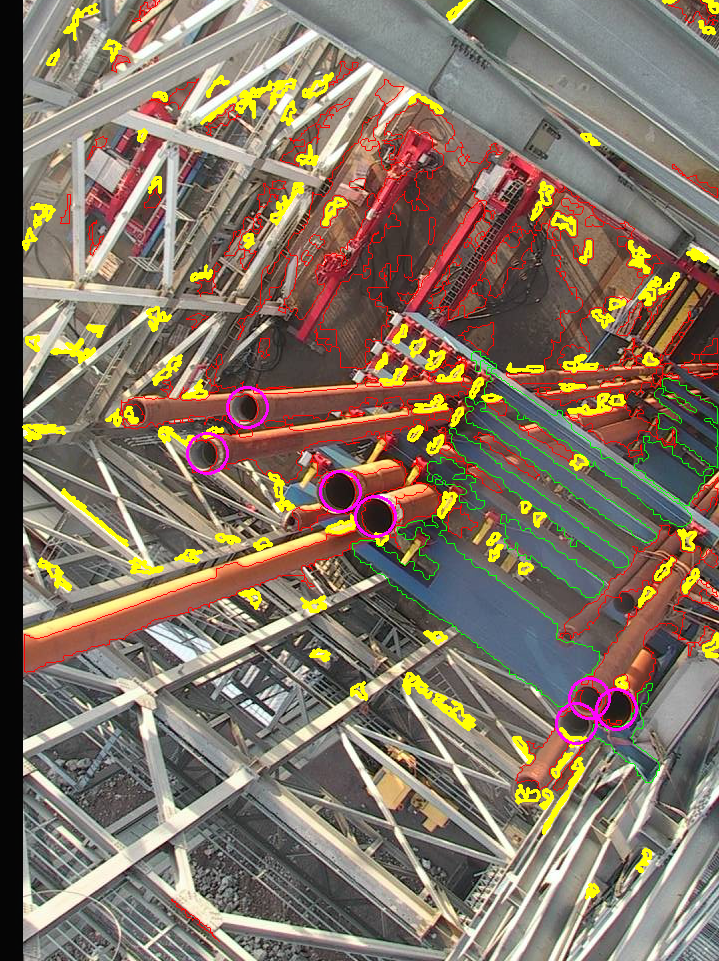
\includegraphics[width=0.8\textwidth]{output.png}
    \caption{The output from the implementation. Source: Own work}
    \label{fig:output}
\end{figure}
\FloatBarrier

\section{Discussion}
\subsection{Auto CCTV tracking}
The C++11-program ran quicker than the Python-program, but it did not seem that using OpenCL had much of an effect on the implementation. Contrary to what was expected, it seems that the OpenCL-accelerated run of the implementation actually increased cycle times and slowed down the program.

Some changes had to be made to the Python version to make it run using OpenCV 3.0.0, in order to have a common ground for testing. It is unknown whether these changes have made the Python implementation slower than when it was used by the author for the work on the unpublished project thesis. Specifically, the video capture was changed to use cv2.videoCapture, instead of a custom-made video capture method. This relies on external libraries.

The reason for the C++11-program to run with a cycle time mean of 43.6120 milliseconds, a lot less than the old Python version that had a cycle time mean of 8302.39 milliseconds, can also be contributed to a different implementation of the FindGlyph-method. The author tried to make the Python and C++-version equal, but in the end, the C++ version made assumptions about the glyph being the largest square in the image whereas the Python version inspects all squares in the image. However, by looking at the Python version grab cycle time, it appears to be mostly the video capture that consumes resources.

Looking at the C++11-program when used with OpenCL, difficulties with getting the T-API to work with all OpenCV-algorithms were encountered. This ended with most of the FindGlyph-method to work with the traditional cv::Mat instead of the new OpenCL-enabled cv::Umat. This explains why no real speedup was found. The process of enabling OpenCL and transferring image data into the GPU makes the program incur some overhead, which can be seen slightly in the cycle time plot.

The C++11-program did however track the glyph well, and were able to follow the glyph as it moved up the linear actuator.

\subsection{Tubular detection}
The program was implemented in Python and used OpenCV 3.0.0, and its output shows that seven out of eleven tubulars were identified properly, which is not great. The detection was a result of blob detection, a simple algorithm that does not use the extra information that is present in the image, including the position of the fingerboard, the tubular pipe walls and fingers found in the fingerboard.

The results show that it is possible to find tubular in a fingerboard using machine vision, however the reliability depends on how well the machine vision is implemented. By having images from several angles, it should be possible to achieve better results. The authors dataset was only from one camera, and the site was unsheltered, which means that snow and lightning effects make the valid dataset even smaller.



\section{Recommendations for future work}
\subsection{Multithreading}
If a function blocks the execution of our single thread, the whole program runs slower, which in turn leads to an increased delay in the control system and may make the auto tracking CCTV system unstable.

By separating functionality into threads that run by themselves and communicate using ZeroMQ or similar software library, a temporary latency spike in the communication between a camera and the software will not slow down the rest of the system.

In order to implement this fully, great care needs to  be taken to ensure that either we wait for all data to be present before we act upon it, or we discard it if it gets delayed too much to ensure a near-realtime behavior.

\begin{figure}[ht]
    \centering
    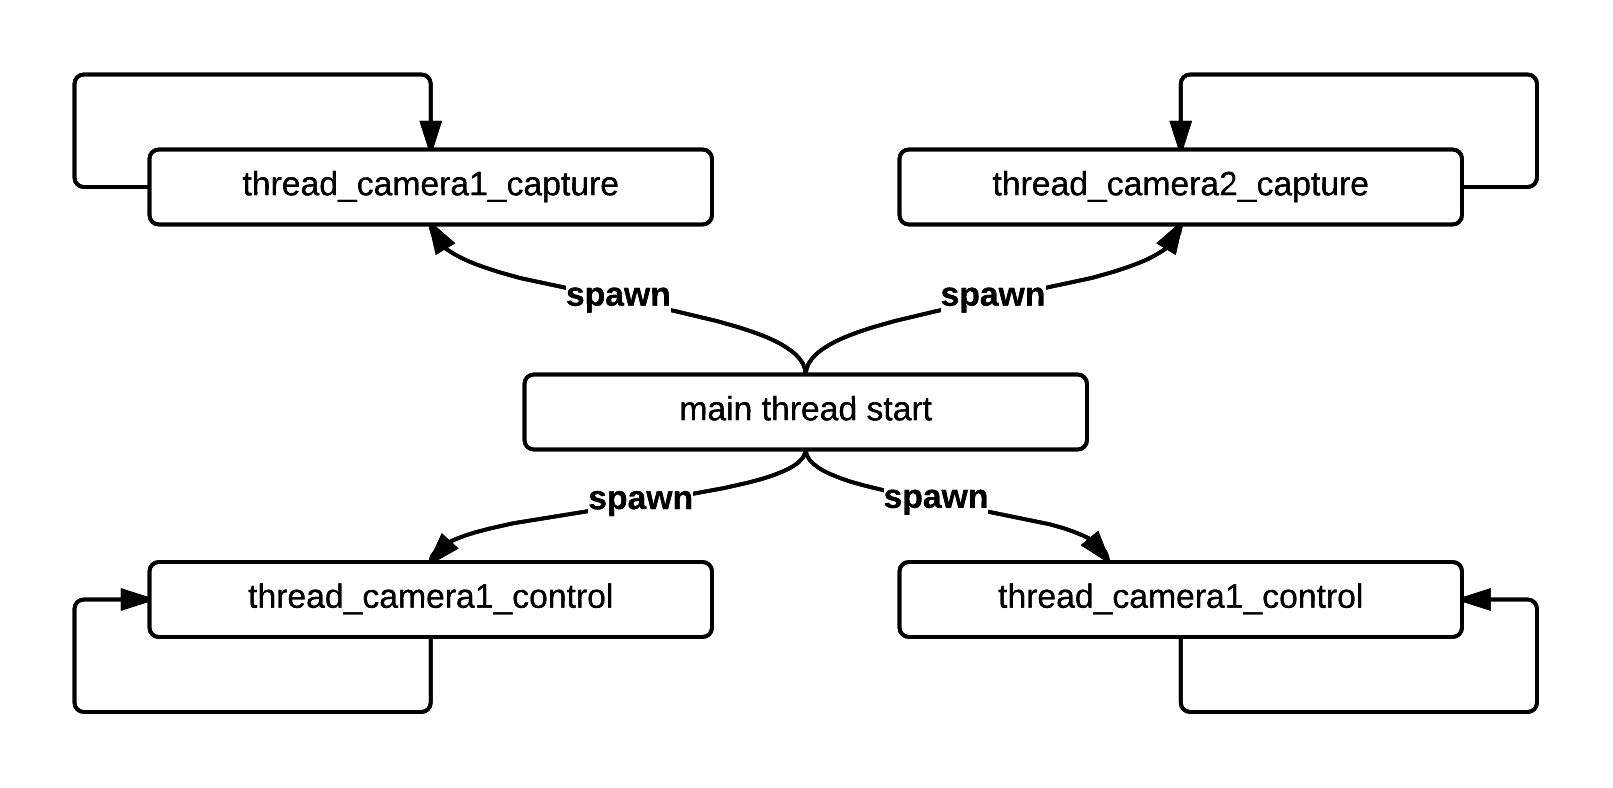
\includegraphics[width=1.0\textwidth]{software_multithread.png}
    \caption{Multithreading concept runs camera capture independent of camera PTZ control. Source: Own work}
    \label{fig:software_multithread}
\end{figure}
\FloatBarrier

\subsection{Augmented Reality}
In order to provide the driller and assistant driller with valuable information, a heads-up display could be used. This could use the video stream from the auto tracking CCTV cameras to overlay useful information depending on where in a sequence the machines are. By augmenting the image with data from both the control system as well as data interpreted from the machine vision system, we may also use data fusion to determine how accurate the displayed data is, and output the best result possible.

\begin{figure}[ht]
    \centering
    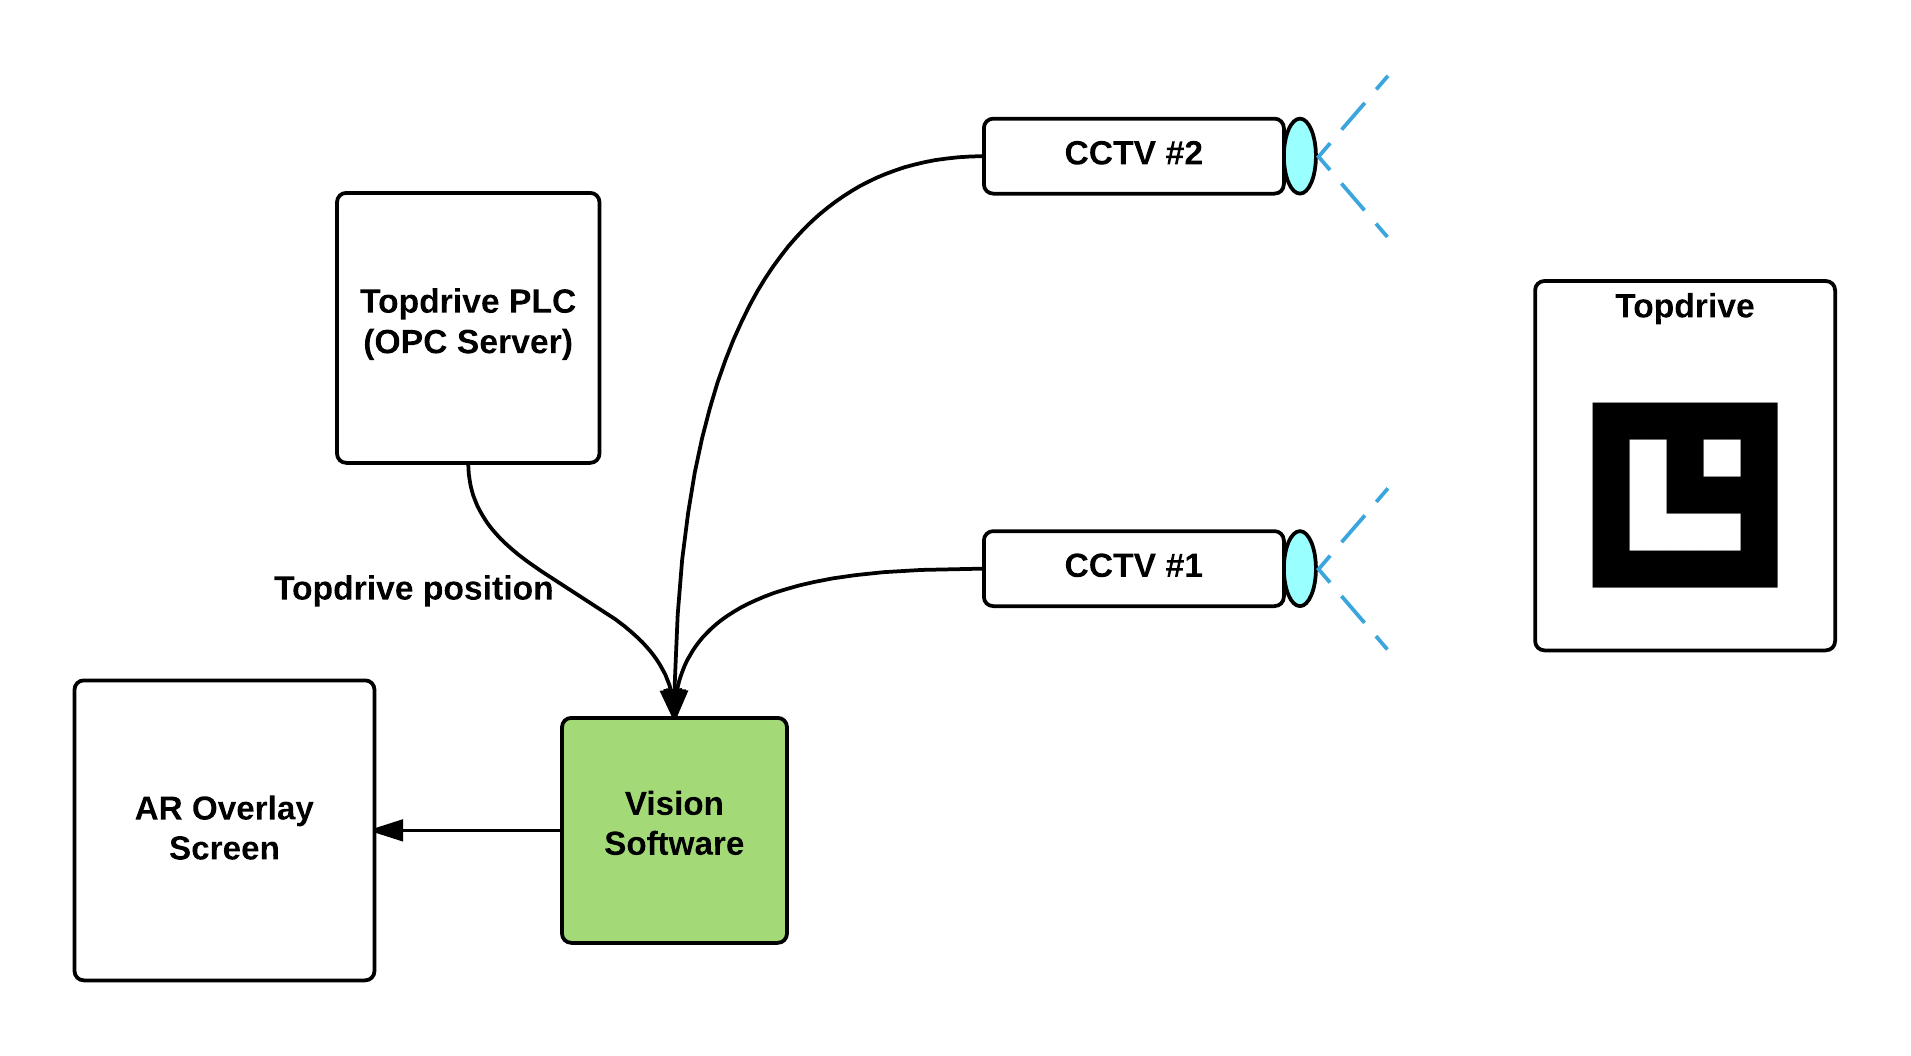
\includegraphics[width=1.0\textwidth]{augmented_data_flow.png}
    \caption{Data fusion using PLC and vision data. Source: Own work}
    \label{fig:augmented_data_flow}
\end{figure}
\FloatBarrier


\begin{figure}[ht]
    \centering
    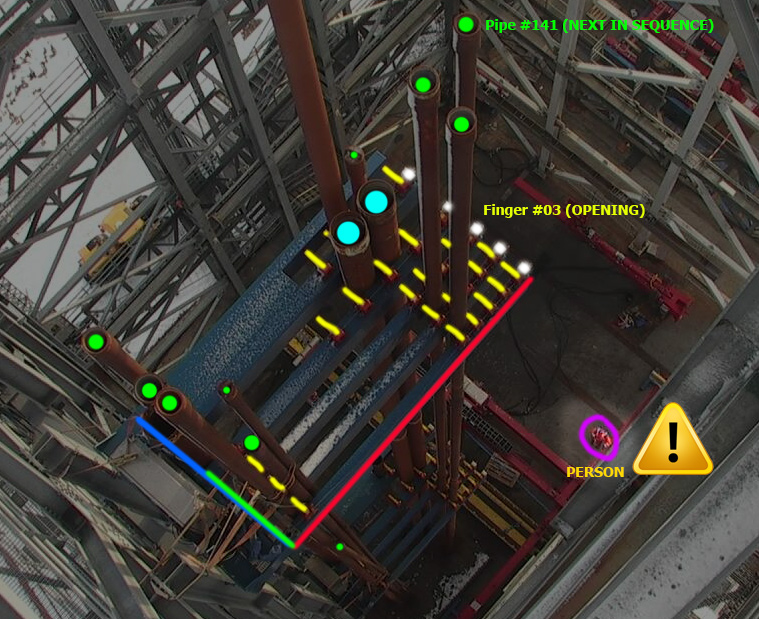
\includegraphics[width=1.0\textwidth]{mockup_augmented_reality.jpg}
    \caption{Fingerboard augmented reality mockup. Source: Own work}
    \label{fig:mockup_augmented_reality}
\end{figure}
\FloatBarrier

\begin{figure}[ht]
    \centering
    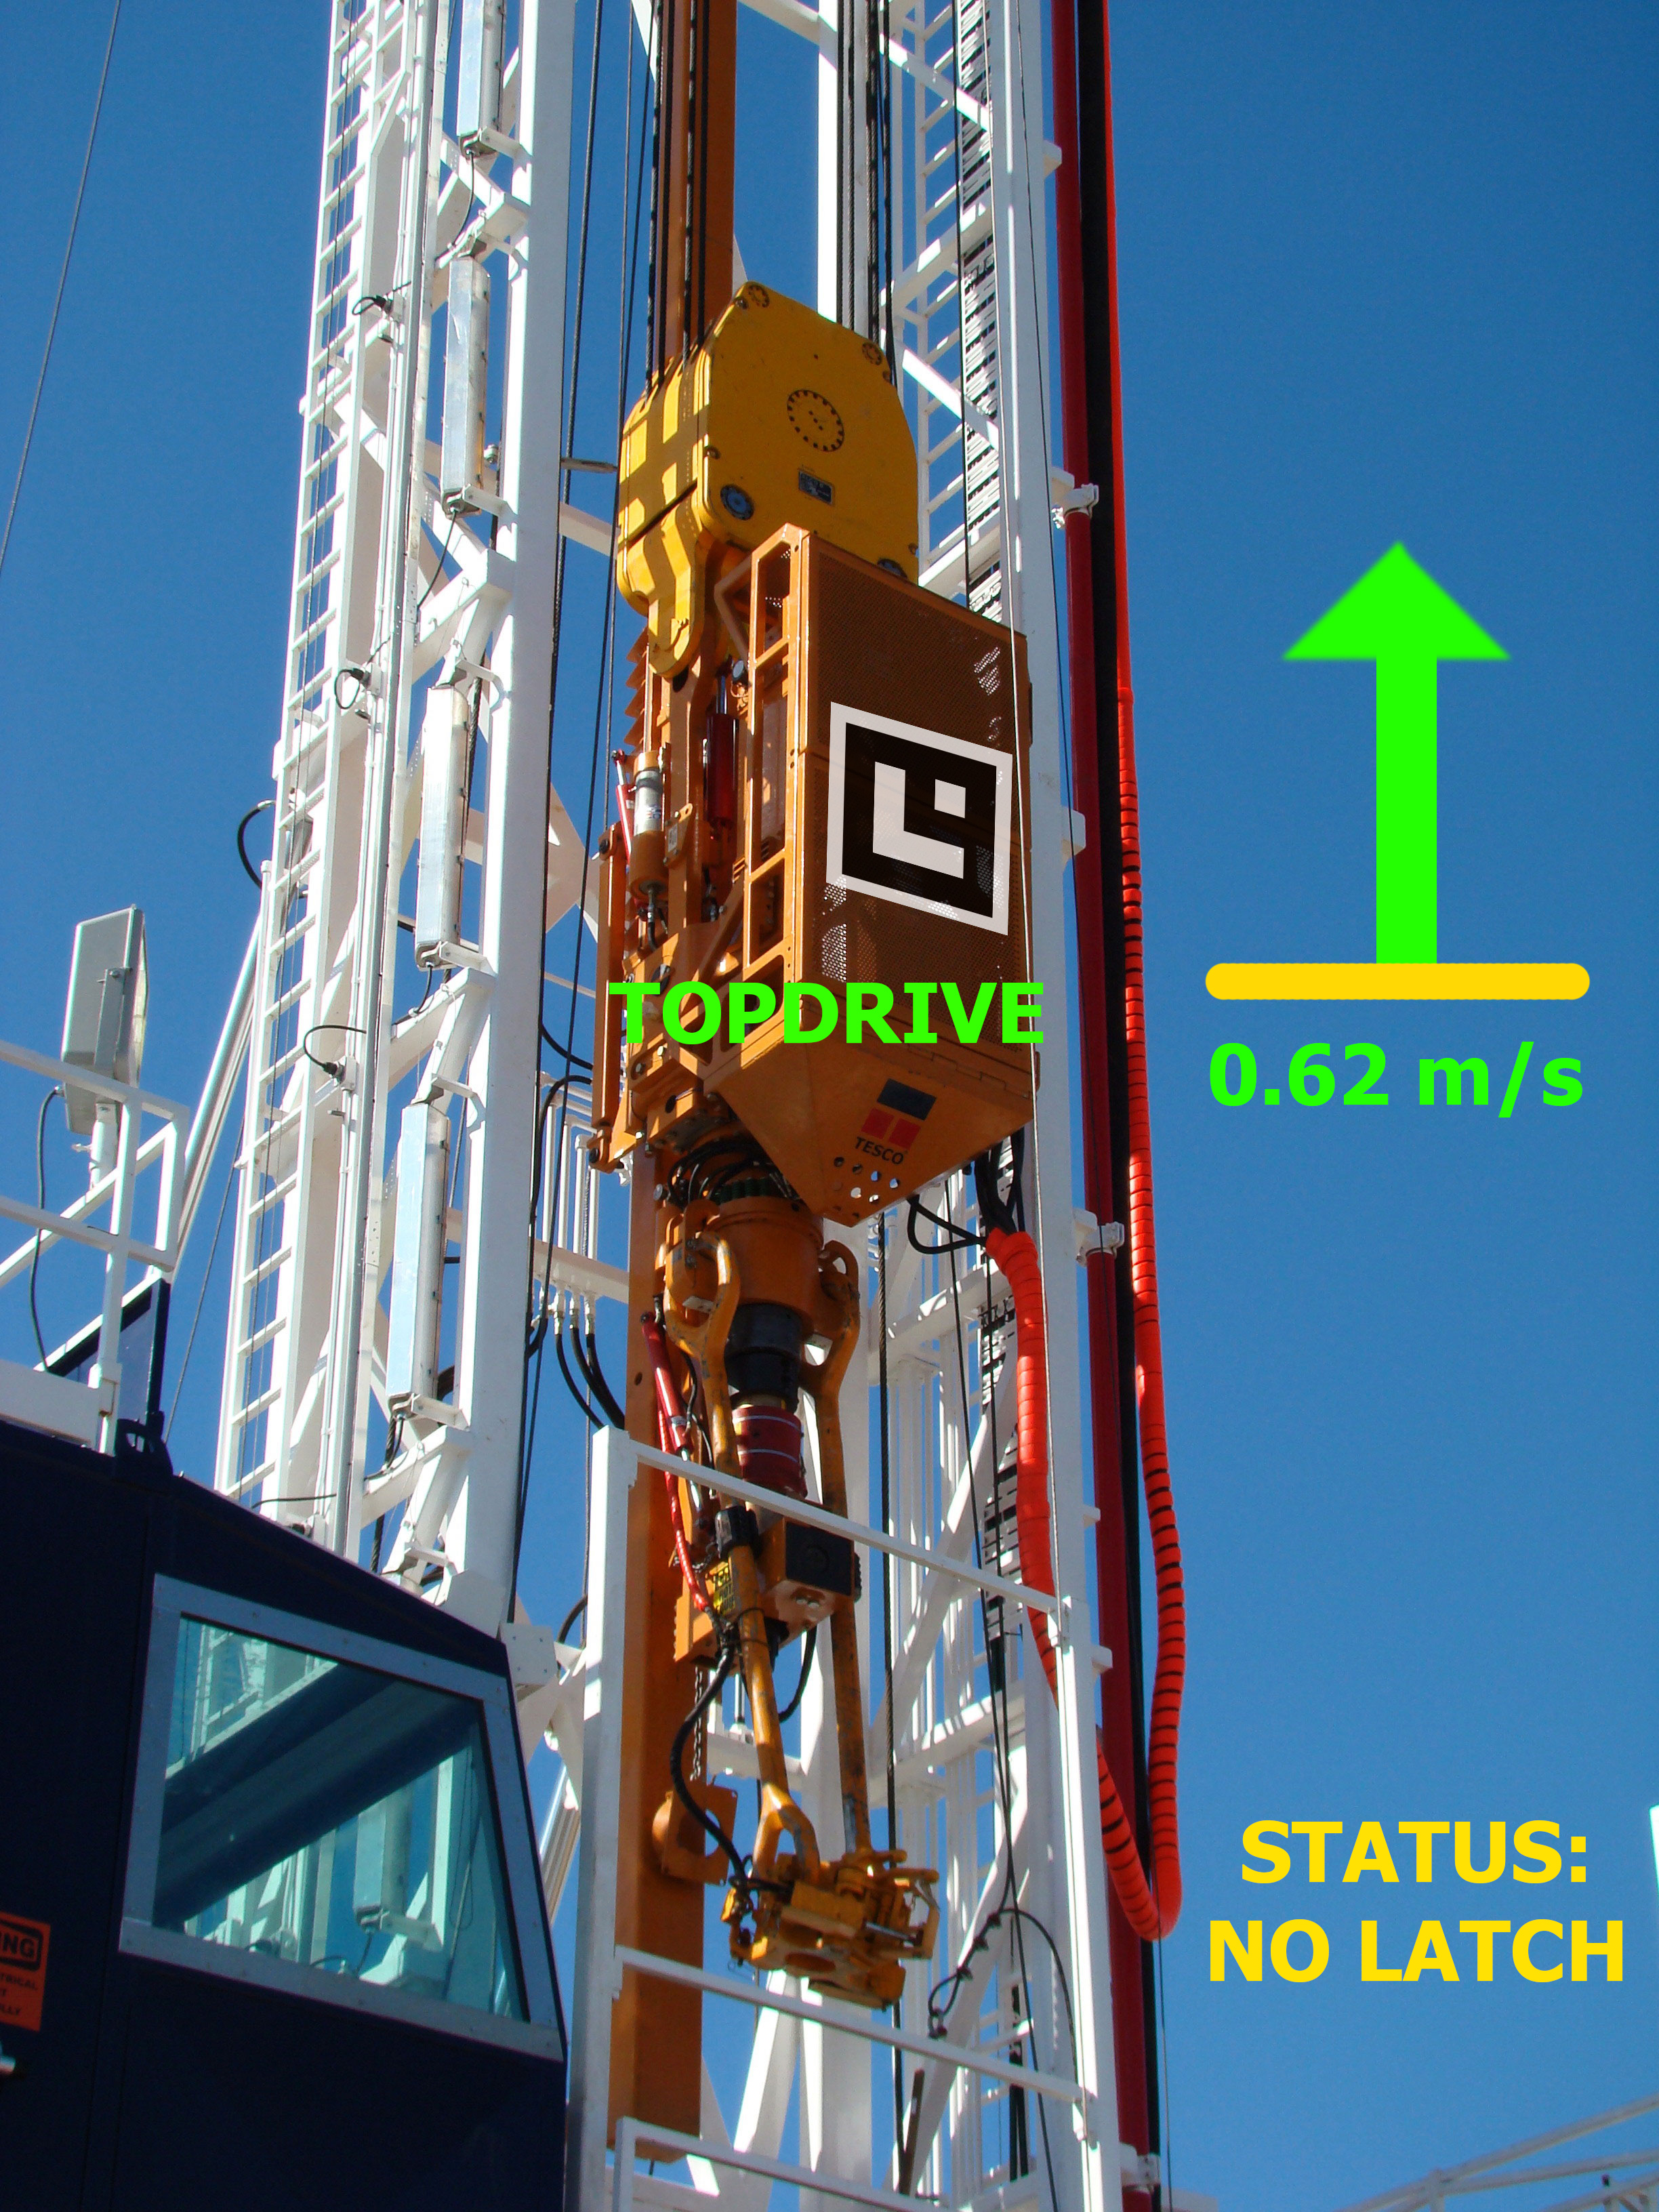
\includegraphics[width=0.8\textwidth]{mockup_augmented_reality_topdrive.jpg}
    \caption{Topdrive augmented reality mockup. Source: \citet{dc15} modified by author}
    \label{fig:mockup_augmented_reality_topdrive}
\end{figure}
\FloatBarrier